\documentclass{article}
\usepackage{graphicx} % Required for inserting images
\usepackage{float} % Required for controlling the position of images

\title{Assignment 3 - Option 1 - DD2424 - K-Layer Network and Batch Normalization}
\author{Tristan Perrot}
\date{April 2024}


\begin{document}

\maketitle
\begin{center}
    
\includegraphics[scale=0.25]{images/KTH_logo_RGB_svart.png}
\end{center}

\section*{Gradient check}

After completing the code for the previous assignment, I have upgraded the code to support a K-layer network. The code is now able to train a K-layer network. This model is without batch normalization and to check whether the gradient computation was good or not I used the same tests as in the previous assignment. \\
\textit{How I checked my analytic gradient computations with batch normalization?} \\
As I did before, for the parameters of the network that are not in the batch normalization I computed numerically the gradient with the given function. Moreover, for the \texttt{gamma} and \texttt{beta} parameters of the batch normalization, I computed the gradient with the grad functionality of PyTorch. I compared the two gradients and they were the same given the relative error (around $10^{-15}$ compared to autograd and $10^{-7}$ compared to numerical). \\

\section*{3 layer network}

\begin{figure}[H]
    \centering
    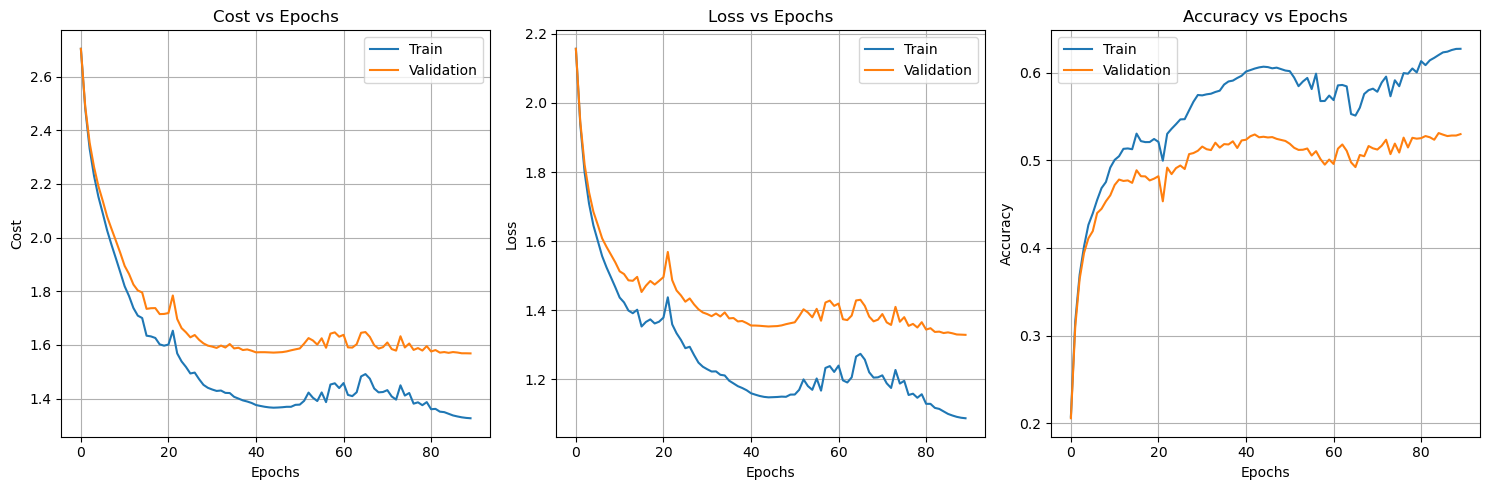
\includegraphics[width=\linewidth]{Result_Pics/3 layer - no BN.png}
    \caption{The training and validation loss for a 3-layer network without batch normalization with \texttt{lambda=.005}. The \textbf{test accuracy} is 53.05\%. I used Xavier initialization.}
\end{figure}

\begin{figure}[H]
    \centering
    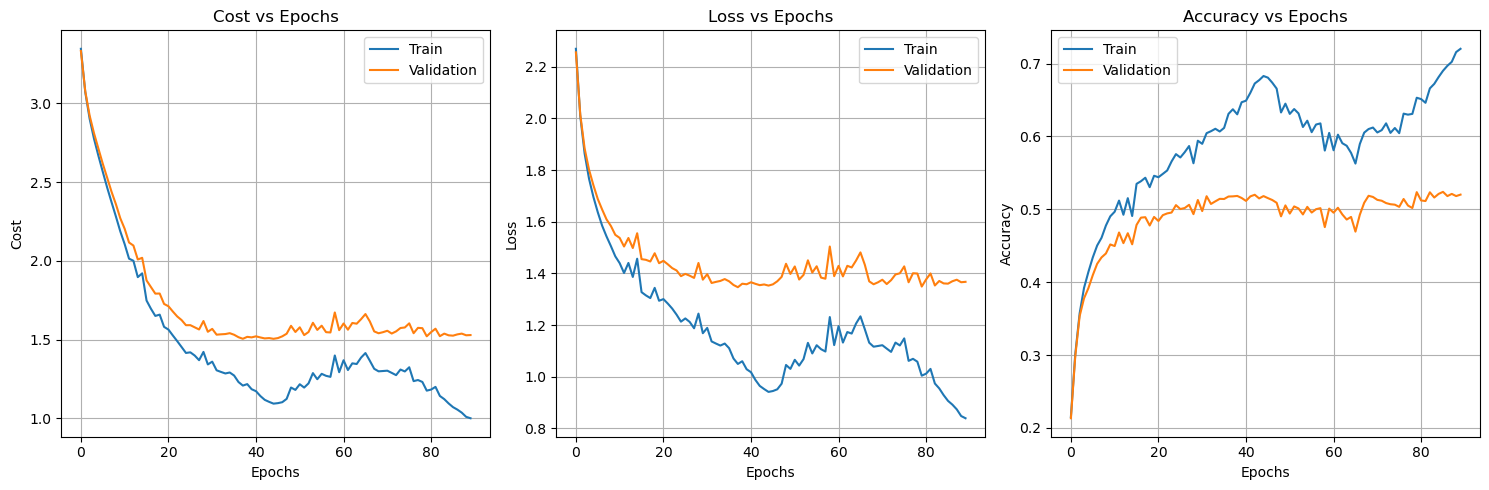
\includegraphics[width=\linewidth]{Result_Pics/3 layer - BN.png}
    \caption{The training and validation loss for a 3-layer network with batch normalization with \texttt{lambda=.005}. The \textbf{test accuracy} is 51.45\%. I used He initialization.}
\end{figure}

Here we can see that the batch normalization helps a lot for the training accuracy. Moreover, with a bit of tuning, the result for the test accuracy will be better. We can see that the loss and the cost are really smaller with batch normalization. The training is also faster. \\

\section*{9 layer network}

\begin{figure}[H]
    \centering
    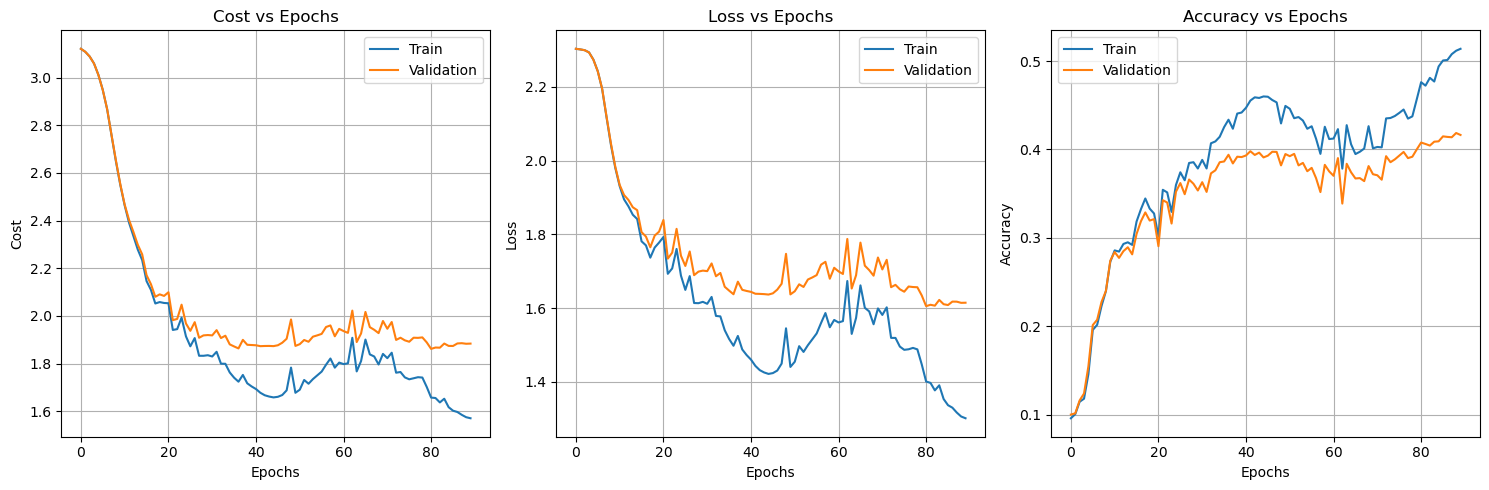
\includegraphics[width=\linewidth]{Result_Pics/9 layer - no BN.png}
    \caption{The training and validation loss for a 9-layer network without batch normalization with \texttt{lambda=.005}. The \textbf{test accuracy} is 42.27\%. I used Xavier initialization.}
\end{figure}

\begin{figure}[H]
    \centering
    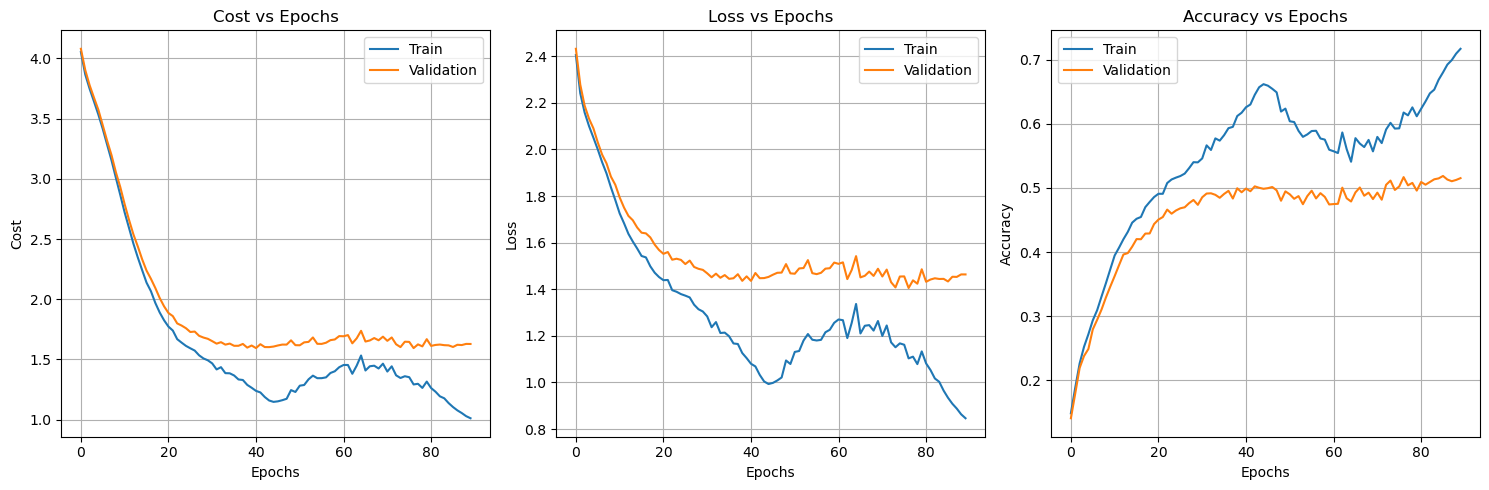
\includegraphics[width=\linewidth]{Result_Pics/9 layer - BN.png}
    \caption{The training and validation loss for a 9-layer network with batch normalization with \texttt{lambda=.005}. The \textbf{test accuracy} is 51.03\%. I used He initialization.}
\end{figure}

Here we can see that the batch normalization helps a lot for the training accuracy. Moreover, the final test accuracy difference is huge ! Almost 10\% of difference. The training is also faster. We can see here the powerfulness of the batch normalization. \\

\section*{Lambda tuning}

I re-used the technique of the previous assignment to tune the lambda parameter. I used the 3-layer network with batch normalization. I tried different values of lambda with \texttt{l\_min=-4} and \texttt{l\_max=-0.3} for the exponential search. I used an higher lambda because we were having great result with \texttt{lambda=.005}. I compared the validation accuracy and each time take the best and the worst lambda from the 5 best training for the next fine tuning. \\
At the end of 3 rows of fine tuning. I get this results: \\
\begin{itemize}
    \item \texttt{lambda=0.01634}, Accuracy: 0.5488
    \item \texttt{lambda=0.02036}, Accuracy: 0.5468
    \item \texttt{lambda=0.0226}, Accuracy: 0.5464
\end{itemize}

\begin{figure}[H]
    \centering
    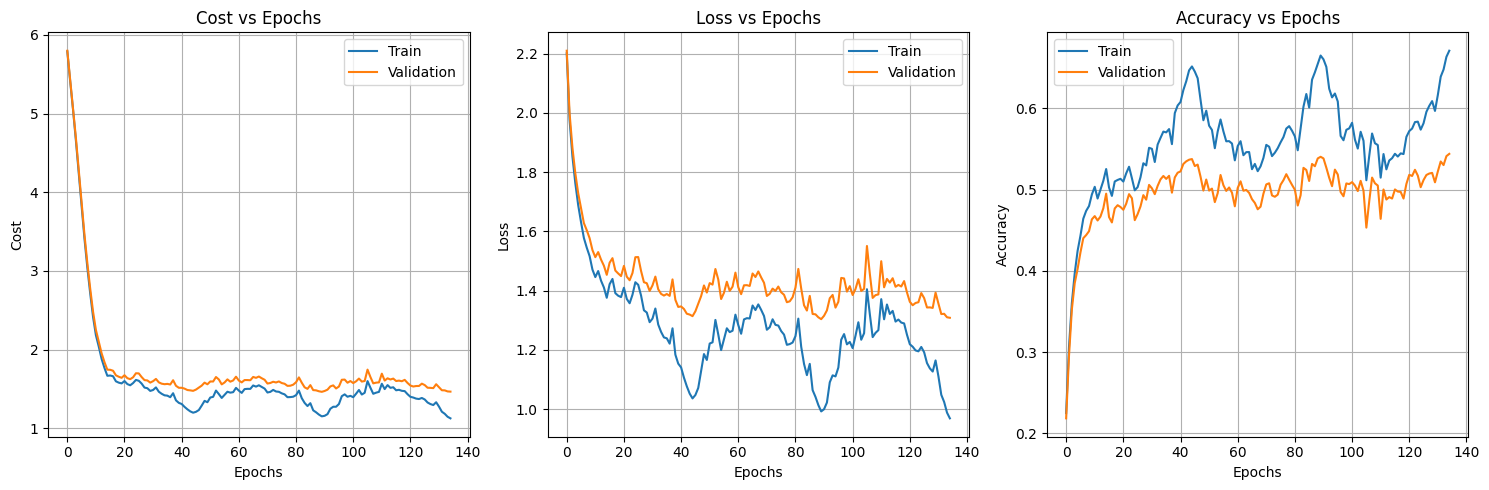
\includegraphics[width=\linewidth]{Result_Pics/3 layer - BN - lambda search.png}
    \caption{The training and validation loss for a 3-layer network with batch normalization with \texttt{lambda=.01634}. The \textbf{test accuracy} is 52.58\%. I used He initialization.}
\end{figure}

There we can see that the test accuracy is 1.13\% better than the previous same model with batch normalization. We can see that the lambda tuning can be really important. \\

And then I used the best lambda and used it for a 9-layer network. The result is:

\begin{figure}[H]
    \centering
    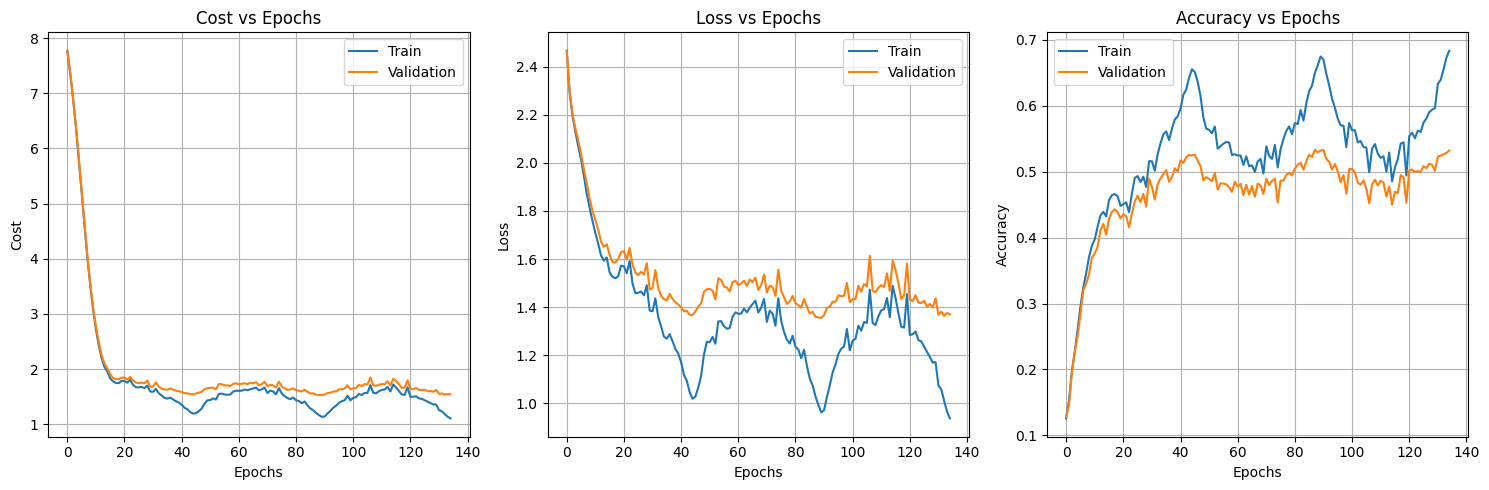
\includegraphics[width=\linewidth]{Result_Pics/9 layer - BN - lambda search.png}
    \caption{The training and validation loss for a 9-layer network with batch normalization with \texttt{lambda=.01634}. The \textbf{test accuracy} is 52.77\%. I used He initialization.}
\end{figure}

Here again we gain 1.74\% of accuracy with the lambda tuning which is really good. \\

\section*{Sensitivity to initialization}

I tested the sensitivity to initialization for the 3-layer network with and without batch normalization by initializing the weights with gaussian distribution with mean 0 and standard deviation of 1e-1, 1e-3, 1e-4. I used \texttt{lambda=.005} for the 3-layer network. \\

\begin{figure}[H]
    \centering
    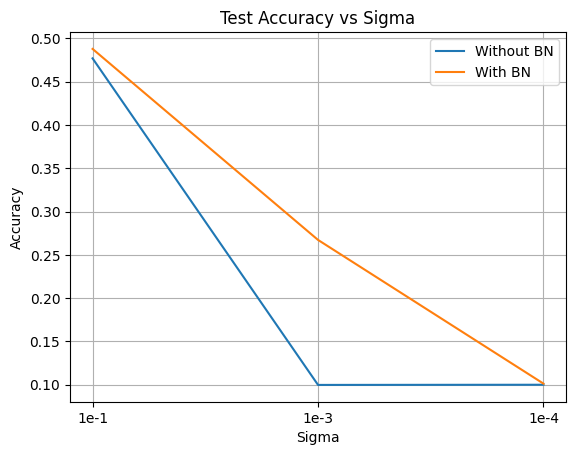
\includegraphics[width=\linewidth]{Result_Pics/sensitivity to initialization.png}
    \caption{Sensitivity to initialization}
\end{figure}

We can see the all the networks are really sensitive to the initialization. Moreover, it is really interesting to see that the network with batch normalization is less sensitive to the initialization. \\

\end{document}